%%%%%%%%%%%%%%%%%%%%%%%%%%%%%%%%%%%%%%%%%%%%%%%%%%%%%%%%%%%%%%%%%%
%%%%%%%% ICML 2015 EXAMPLE LATEX SUBMISSION FILE %%%%%%%%%%%%%%%%%
%%%%%%%%%%%%%%%%%%%%%%%%%%%%%%%%%%%%%%%%%%%%%%%%%%%%%%%%%%%%%%%%%%

% Use the following line _only_ if you're still using LaTeX 2.09.
%\documentstyle[icml2015,epsf,natbib]{article}
% If you rely on Latex2e packages, like most moden people use this:
\documentclass{article}

% use Times
\usepackage{times}
% For figures
\usepackage{graphicx} % more modern
%\usepackage{epsfig} % less modern
\usepackage{subfigure} 

% For citations
\usepackage{natbib}

% For algorithms
\usepackage{algorithm}
\usepackage{algorithmic}

% As of 2011, we use the hyperref package to produce hyperlinks in the
% resulting PDF.  If this breaks your system, please commend out the
% following usepackage line and replace \usepackage{icml2015} with
% \usepackage[nohyperref]{icml2015} above.
\usepackage{hyperref}

% Packages hyperref and algorithmic misbehave sometimes.  We can fix
% this with the following command.
\newcommand{\theHalgorithm}{\arabic{algorithm}}

% Employ the following version of the ``usepackage'' statement for
% submitting the draft version of the paper for review.  This will set
% the note in the first column to ``Under review.  Do not distribute.''
%\usepackage{icml2015} 

% Employ this version of the ``usepackage'' statement after the paper has
% been accepted, when creating the final version.  This will set the
% note in the first column to ``Proceedings of the...''
\usepackage[accepted]{icml2015}
%\usepackage[brazilian]{babel}
\usepackage[utf8]{inputenc}
\usepackage[T1]{fontenc}




% The \icmltitle you define below is probably too long as a header.
% Therefore, a short form for the running title is supplied here:
\icmltitlerunning{AM no futebol }

\begin{document} 

\twocolumn[
\icmltitle{Métodos de Aprendizado de Máquinas aplicado à predição de jogos de futebol}

% It is OKAY to include author information, even for blind
% submissions: the style file will automatically remove it for you
% unless you've provided the [accepted] option to the icml2015
% package.
\icmlauthor{Felipe Augusto Pereira Fernandes}{felipeapfernandes@gmail.com}
\icmladdress{CEFETMG}


% You may provide any keywords that you 
% find helpful for describing your paper; these are used to populate 
% the "keywords" metadata in the PDF but will not be shown in the document
\icmlkeywords{machine learning, prediction, soccer}

\vskip 0.3in
]

%\begin{abstract} 
%The purpose of this document is to provide both the %basic paper template and
%submission guidelines.
%\end{abstract}


\begin{abstract}
	Futebol é considerado o esporte mais popular do mundo \cite{federation2007fifa}. Por isto, é muito comum vermos pessoas discutindo em reuniões familiares e mesas de bar sobre quem vai ganhar uma partida. Analisando os resultados dos jogos das equipes é possível estabelecer um histórico de desempenho durante a temporada. Este trabalho estuda algoritmos de aprendizado de máquina para prever o resultado de uma partida de futebol: vitória do mandante, empate
	ou vitória do visitante. A partir de dados básicos de desempenhos e com entradas que tentam capturar as influências da dinâmica de uma partida de futebol, este trabalho tem o objetivo de estudar o desempenho dos algoritmos de aprendizado de máquina aplicados a predição de jogos de futebol, utilizando uma base de dados pública, \cite{database}, que contêm informações de jogos de 8 países. 
	
	\textbf{Keywords}: Soccer match prediction, Pattern Classification, Machine Learning, Football.
\end{abstract}

\section{Introdução}

Futebol é o esporte mais popular do mundo e no Brasil
não é diferente. Futebol é um assunto sempre presente em
mesas de bares, reuniões familiares e grupos de amigos. Qual
time vai ganhar a partida? Quem vai vencer o campeonato?
Qual time é melhor? são indagações sempre presentes nas
conversas. Justamente por isso, veículos de comunicação como
jornais e programas de televisão sempre possuem especialistas
para discutir e fazer projeções, empirícas, sobre quem serão
os vencedores dos jogos da rodada do campeonato.

Determinar o resultado de uma partida não é uma tarefa
simples, pois o futebol é um esporte coletivo sujeito a inúmeras
variáveis, como padrão de um time, esquema tático, falhas
individuais de jogadores, capacidade de execução e habilidade
dos jogadores, condição do gramado, motivação da equipe,
montagem da equipe, árbitros  etc. 

Um estudo, apresentado em \textit{ The numbers game: why
everything you know about football is wrong} \cite{anderson2013numbers} e feito com
mais de dez mil jogos, mostra que a média de gols por partida
vem mudando ao longo dos anos. Atualmente, essa média é
de 2.6 gols por jogo. A Figura \ref{fig:gols_ingles} mostra o comportamento desta média nas temporadas do campeonato inglês da primeira divisão desde 1940 a 2014.

\begin{figure}[!h]
	\centering
	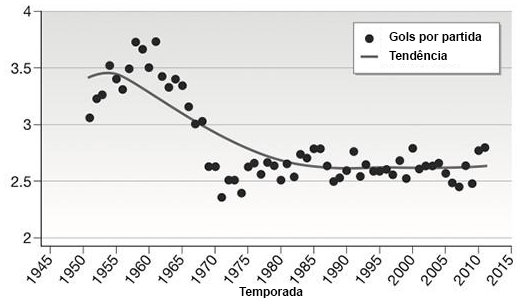
\includegraphics[width=0.45\textwidth]{./04-figuras/ingles_gols_2.png}
	\caption{Média de gols em uma partida ao longo dos anos.}
	\label{fig:gols_ingles}
\end{figure}





Ao analisar os resultados dos jogos das equipes durante
uma temporada é possível estabelecer um histórico de desempenho, como quantidade de gols marcado, gols sofrido, quantidade de vitórias, derrotas, empates e etc. A partir destes valores é possível perceber que diferentes times apresentam valores próximos em momentos distintos do campeonato, quando os valores comparados são divididos pela quantidade de jogos já realizados. Desta forma, é possível estabelecer o padrão de um
time em um determinado jogo em uma determinada rodada em
um campeonato.

Estatísticas de jogos, times e jogadores são utilizadas no auxílio a determinação
de resultados de jogos de futebol. Hoje existem sites especializados em estatísticas,
que vem sendo amplamente divulgados em programas de televisão e em transmissão
de jogos. Analisando os resultados dos jogos das equipes é possível estabelecer um
histórico de desempenho durante a temporada. Quando os números das equipes são analisados percebe-se que podemos descrever uma partida de futebol com esses números de ambas as equipes.

Este artigo propõe o estudo de modelos de aprendizado de máquina para a predição de jogos de futebol. Estudar seus impactos e performance em cima da base de dados pública. Além disso, este artigo visa a consolidação dos estudos na disciplina de aprendizado de máquina, cursada no mestrado em modelagem e matemática computacional do CEFETMG. 


\section{Trabalhos relacionados}

Apesar da grande popularidade do esporte, existem poucos trabalhos científicos
dedicados à predição de jogos de futebol \cite{aslan2007comparative} . Em Cheng et
al.\cite{cheng2003new}, os autores demonstram o bom desempenho da utilização de Redes Neurais Artificiais (RNAs) para a predição de resultados de jogos de futebol. No trabalho, as RNAs implementadas são comparadas a métodos estatísticos, apresentando taxas de acerto superiores.
Cheng et al. \cite{cheng2003new} propõem o uso de RNAs para a predição de jogos de futebol.
A Figura \ref{fig:cheng_modelo} exemplifica o modelo proposto. O modelo baseou-se em uma abordagem hibrida, criando um sistema que primeiramente avalia o nível dos times, separando os jogos em 3 conjuntos: quando o time mandante é melhor, times de níveis iguais e o time visitante é melhor. Para isto foi utilizado a diferença da média de pontos e a diferença da média de gols feitos pelas equipes. Para o cálculo da média de pontos, calcula-se os pontos dos times na competição até uma determinada rodada. Para cada vitória soma-se três pontos, para cada empate um ponto e zero pontos para a derrota. Ao final, divide-se a quantidade de pontos somados pela quantidade de jogos disputados pelo time. A média de gols feitos pelas equipes é calculada somando os gols feitos até determinada rodada e então divide-se esta soma pela quantidade de jogos disputados.Cada entrada da rede passa por este mecanismo seletor que define a qual RNA aquele jogo pertence. O modelo de entrada utilizado pelos autores é apresentado na Figura \ref{fig:cheng_entradas}.

\begin{figure}[!h]
	\centering
	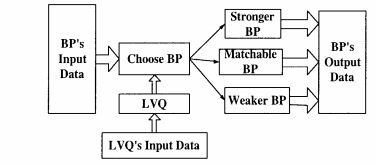
\includegraphics[width=0.48\textwidth]{./04-figuras/cheng_modelo.JPG}
	\caption{Architecture model proposed by Cheng et al. \cite{cheng2003new}}
	\label{fig:cheng_modelo}
\end{figure}  


Para o treinamento eles utilizaram os dados do campeonato italiano da tempo-
rada 2001-2002, com 34 rodadas. Inicialmente foram utilizados os dados da rodada 7
até a rodada 17 para treinamento. O teste foi feito com os jogos da rodada 18 até a 34. Entretanto o teste foi feito rodada a rodada, somando 17 taxas de acertos, uma para cada rodada. Ou seja, para o teste da rodada 20, os dados dos jogos até a rodada 19 foram utilizados para o treinamento da rede, e a taxa de acerto foi coletada, utilizando sempre
9 jogos para realizar o teste. Os jogos das 6 primeiras rodadas não foram utilizados no processo de treinamento da rede nem de teste já que os autores acreditam que os primeiros jogos estão muito mais sujeitos às aleatoriedades do futebol.

A saída dessa rede híbrida seria a predição do resultado do jogo como vitória
mandante, empate ou vitória do visitante. Este modelo proposto atingiu um taxa de
acerto de 52.29\% sendo melhor que os métodos de previsão estatísticos existentes, tais como Elo Rating \cite{Elo}. Entretanto Cheng et al. \cite{cheng2003new} apontam o fato de que as últimas seis rodadas apresentaram uma taxa de acerto de 44.77\%, justificando esta porcentagem ao número limitado de jogos para o treinamento e a fatores acidentais a que o futebol está sujeito.


Aslan e Inceoglu \cite{aslan2007comparative} fizeram um comparativo de modelos de previsão de resultados de jogos de futebol. Ao fim propuseram um novo modelo de rede, baseando somente no desempenho de cada time como mandante e visitante. Para isso, eles simplesmente incrementam uma variável para cada vitória, decrementam para cada derrota e em caso de empate não alteram o valor da variável. Foram propostos então dois modelos de entradas para redes Learning Vector Quantization (LVQ): uma somente com os dados de desempenho como mandante para o time mandante e os dados de desempenho como visitante para o time visitante; e outra com os dados de mandante e visitante para ambos os times. Os processos de treinamento e teste foram idênticos aos propostos por Cheng et al. \cite{cheng2003new}. A rede com menos entradas teve 53.25\% de taxa de acerto contra 51.29\% do outro modelo. Os autores concluíram que a modelagem dos dados de entrada da RNA é um problema crítico.

\begin{figure}[!h] \centering
	%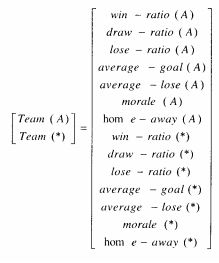
\includegraphics[width=0.3\textwidth]{./04-figuras/cheng_entrada.jpg}
	
	$$
	\begin{array}{ccc}
	
	\left[ \begin{array}{c}
	Team (A) \\
	Team (*)
	\end{array} \right]
	
	=
	
	\left[ \begin{array}{c}
		 win - ratio (A)   \\
		 draw - ratio (A)  \\
		 lose - ratio (A)  \\
		average - goal (A) \\
		average - lose (A) \\
		    morale (A)     \\
		hom \ e - away (A) \\
		 win - ratio (*)   \\
		 draw - ratio (*)  \\
		 lose - ratio (*)  \\
		average - goal(*)  \\
		average - lose(*)  \\
		    morale (*)     \\
		hom \ e - away (*)
	\end{array} \right]
	
	\end{array} 
	$$
	
	\caption{Modelo de entrada proposto por Cheng et al. \cite{cheng2003new}}
	\label{fig:cheng_entradas}
\end{figure} 


\section{Base de dados}
Para este estudo uma base de dados pública foi utilizada. Ela está disponível no \textit{site} kaggle \cite{database}. Nesta base de dados tem mais de 25000 partidas, onde tem informação de mais de 10000 jogadores de 11 países com seus principais campeonatos. Esta base de dados também tem informação sobre as escalações e posições dos jogadores( coordenadas X e Y) e valores dos prêmios pagos pelas casas de apostas para vitória do mandante, empate e vitória do visitante.

Esses dados estão representados em sete tabelas: \textit{Country}, \textit{League}, \textit{Match}, \textit{Player}, \textit{Player Attribute}, \textit{Team} e \textit{Team\_Attributes}.

\section{Modelagem}

Como o futebol é um esporte coletivo, suscetível a várias aleatoriedades, no
qual fatores físicos, técnicos e psicológicos influenciam no desempenho de uma equipe, mensurar a qualidade de uma equipe, transformando essa qualidade em um número, é algo altamente subjetivo e complicado.

Em um jogo de futebol pode-se dividir uma equipe em três setores: defesa, meio
de campo e ataque. Em geral, os especialistas afirmam que times com defesa e meio de campo fortes tendem a sofrer menos gols, enquanto times com ataque e meio de campo fortes tendem a fazer muitos gols. Portanto, indicadores de qualidade da defesa, meio de campo e ataque dos times parecem ser entradas interessantes para a modelagem desse problema. Baseado em especialistas, discretiza-se a qualidade das equipes, conseguindo fazer uma comparação da qualidade das mesmas.

Para obter esses valores, foram utilizados os indicadores de qualidade de defesa,
meio de campo e ataque da franquia de jogos da EA Sports (Electronic Arts Sports), o FIFA. Nele, os jogadores são avaliados de 0 a 100 em diversos atributos
físicos, técnicos e psicológicos. O índice do time é calculado como a média dos atributos de todos os jogadores da equipe. Desta forma, o índice de defesa do time é calculado pela média dos índices defensivos de todos os jogadores da equipe, o índice de meio de campo do time pela média dos atributos de meio de campo e o índice de ataque do time pela média dos atributos de ataque dos jogadores.

É sabido que o mando de campo tem influência no desempenho de um time,
pois jogar ao lado de sua torcida ou sob a pressão da torcida adversária exerce um
efeito psicológico no time. Portanto para a predição de um jogo é interessante avaliar o desempenho do time mandante nos jogos em que ele atuou em casa e o desempenho do time visitante nos jogos em que atuou fora de casa.

No futebol suspensões, lesões e transações de jogadores entre equipes é algo
muito comum durante um campeonato. A mudança de um elenco durante um campeonato pode afetar o desempenho da equipe. Para que a rede seja capaz de captar essas variações é interessante levar em consideração o desempenho da equipe nos últimos
jogos.

Em relação ao impacto da suspensão, lesões e transferência de jogadores, avaliar a performance de um time desde o ínicio da temporada não parece ser a melhor maneira.

Se colocarmos esses indicadores estatisticos de desempenho e analizarmos a performance de uma forma mais local, nos últimos 5 jogos, parece ser mais interessante, visto que esses indicadores mudam de valor quando aplicamos essa janela de tempo no desempenho.

Analizando localmente parece ser mais fácil predizer um próximo comportamento. A figura \ref{fig:liv_goals_scored}
demonstra os gols por jogo de uma forma global, desde o ínicio da temporada. Já a figura \ref{fig:liv_goals_scored5} demonstra o indicador gols a favor por jogo de uma forma local, considerando somente os últimos 5 jogos. As figuras esclarecem essa diferença nos valores dos índices quando aplicamos essa janela de tempo no desempenho.

\begin{figure}[!h]
	\centering
	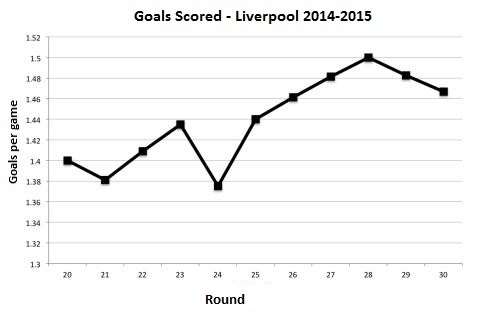
\includegraphics[width=0.45\textwidth]{./04-figuras/Gols_feitos.JPG}
	\caption{Gols marcado por Liverpool na temporada 2014-2015.}
	\label{fig:liv_goals_scored}
\end{figure}

\begin{figure}[!h]
	\centering
	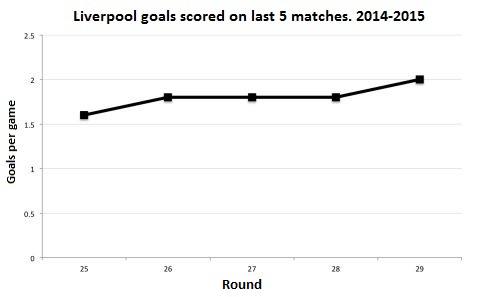
\includegraphics[width=0.45\textwidth]{./04-figuras/Gols_feitos_5jogos.JPG}
	\caption{Gols marcados por jogo nos últimos 5 jogos do Liverpool na temporada 2014-2015.}
	\label{fig:liv_goals_scored5}
\end{figure}


No campo date, foi calculado a diferença em dias do jogo em questão para o ultimo jogo de ambas as equipes, criando assim uma data para o mandante e uma para o visitante.

Portanto estas ideias expostas nesta seção farão parte da descrição de uma partida de futebol.



\section{Metodologia}
Para este trabalho irei aplicar o algoritmo de regressão logistica, \textit{KNeighbors}, \textit{Random Forest} e \textit{Gradient Boosting} ao dado extraído da base de dados.

Jogos dos campeonatos inglês, alemão, francês, espanhol, italiano e português foram utilizados, da temporada 2010-2011 até 2015-2016.

Após aplicar os dados puros da tabela
\textit{Match} irei aplicar um \textit{Feature Engineering} para extrair mais features dos dados presentes nas outras tabelas.

Primeiramente usaremos somente os dados disponiveís na tabela \textit{Matches} para fazermos a descrição de uma partida de futebol. Selecionei todos os jogos onde eu tivesse informação de todos os jogadores da partida e que tivesse dado a respeito do prêmio pago pela casa de aposta Bet365.

Após essa primeira filtragem, foram excluidos os dados referentes aos incidentes da partida, pois poucos jogos continham alguma informação, em formato XML, nestes campos.

Depois uma transformação de variáveis categoricas - \textit{date}, \textit{season}- para ordinal foram feitas.

Por fim, inclui uma coluna referente a classe do jogo: 'H' para vitória do mandante, 'D' para empate e 'A' para vitória do visitante.

Esses dados são compostos pelas seguintes caracteristicas:

	 'country\_id', 'league\_id', 'season', 'stage',  'date', 'match\_api\_id', 'home\_team\_api\_id',  'away\_team\_api\_id', 'home\_player\_X1', 'home\_player\_X2', 'home\_player\_X3', 'home\_player\_X4', 'home\_player\_X5', 'home\_player\_X6', 'home\_player\_X7', 'home\_player\_X8', 'home\_player\_X9', 'home\_player\_X10', 'home\_player\_X11', 'away\_player\_X1', 'away\_player\_X2', 'away\_player\_X3', 'away\_player\_X4', 'away\_player\_X5', 'away\_player\_X6', 'away\_player\_X7', 'away\_player\_X8', 'away\_player\_X9', 'away\_player\_X10', 'away\_player\_X11', 'home\_player\_Y1', 'home\_player\_Y2', 'home\_player\_Y3', 'home\_player\_Y4', 'home\_player\_Y5', 'home\_player\_Y6', 'home\_player\_Y7', 'home\_player\_Y8', 'home\_player\_Y9', 'home\_player\_Y10', 'home\_player\_Y11', 'away\_player\_Y1', 'away\_player\_Y2',
	'away\_player\_Y3',
	'away\_player\_Y4', 'away\_player\_Y5', 'away\_player\_Y6', 'away\_player\_Y7', 'away\_player\_Y8', 'away\_player\_Y9',
	'away\_player\_Y10', 'away\_player\_Y11', 'B365H','B365D', 'B365A' e 'Output' como feature final da classe.


Aplicando esses dados diretamente numa regressão logística, foi atingido uma acurácia de 46.02\%, usando k-fold cross validation com k=10.

Como podemos observar, existem duas features de coordenada para cada jogador num time. Podemos transformar estas 22 features em 2, somente transformando-as na feature formation, que contém número de jogadres na defesa, meio de campo e ataque.

Após essa transformação, denominamos esse conjunto de features e dado como dados-cru. As features do dados-cru são: 'country\_id', 'league\_id', 'season', 'stage', 'date', 'match\_api\_id', 'home\_team\_api\_id', 'away\_team\_api\_id','formation\_home', 'formation\_away', 'B365H', 'B365D', 'B365A' com 'Output' como feature final da classe.

Utilizando regressão logistica, os dados crus apresentaram acurácia média de  46.53\%, using a k-fold validation with k=10.

\subsection{Feature Engineering e Preração dos dados}

Como parte do feature engineering os jogos das 5 primeiras rodadas não foram utilizados para como exemplos, jogos a serem descritos pelas features propostas. O motivador para tal descarte foi o fato de acreditar que nesses jogos os times estão em processo de adaptação, tanto em relação ao campeonato, quanto aos seus novos companheiros, fato que pode tornar os resultados mais aptos a aleatoriedade dos jogos de futebol. Ao desconsiderar este período de adaptação é esperado que a sequência dos resultados seja mais estável em relação ao padrão definido dos times de uma determinada partida. Vale a pena ressaltar que a escolha da quantidade de rodadas
a serem descartadas foi completamente empírica.

A cada jogo de uma rodada é levado em consideração todos os jogos das rodadas
anteriores daquela equipe. Por exemplo, em um jogo da rodada 30, os dados presentes na entrada da rede para este jogo, sofrem influências da rodada 1 à rodada 29.
Tomando como exemplo o jogo Liverpool vs Manchester United disputado no dia 22/03/2015, pertencente a trigésima rodada da temporada 2014-2015, a Figura \ref{fig:ex_rodada29}
demonstra o desempenhos dos times até a vigésima nona rodada.

\begin{figure}[!h]
	\centering
	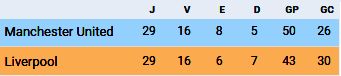
\includegraphics[width=0.45\textwidth]{./04-figuras/Exemplo_Rodada29_2.png}
	\caption{Desempenho de Liverpool e Manchester United em vinte nove jogos}
	\label{fig:ex_rodada29}
\end{figure}

A Figura \ref{fig:Liv_rodada29} e a Figura \ref{fig:ManUtd_rodada29} demonstram o desempenho de Liverpool e Manchester United, respectivamente, ao longo de vinte nove jogos e o desempenho em casa e fora.
Na Figura \ref{fig:Liv_rodada29} J representa o número de jogos, V o número de vitórias, E o número de empates, D o número de derrotas, GP o número de gols feitos e GC o número de gols sofridos. De forma análoga JC significa jogos em casa, VC vitória em casa etc. O mesmo é válido para F, onde JF representa jogos fora, VF vitórias fora etc.

\begin{figure}[!h]
	\centering
	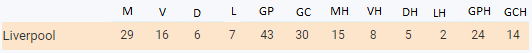
\includegraphics[width=0.45\textwidth]{./04-figuras/Liverpool_30.png}
	\caption{Desempenho detalhado do Liverpool em vinte nove jogos}
	\label{fig:Liv_rodada29}
\end{figure}

\begin{figure}[!h]
	\centering
	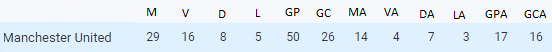
\includegraphics[width=0.45\textwidth]{./04-figuras/ManUtd_30.png}
	\caption{Desempenho detalhado do Manchester United em vinte nove jogos}
	\label{fig:ManUtd_rodada29}
\end{figure}

Para gera estes índices é necessário fazer consultas na tabela Matches e calcular estas taxas.

Também extraí dados das tabelas Team\_attributes, Team, Player e Player\_Attribute.  

Com isso contruí features que eu optei por separar em classes: Base, gols, estilo de jogo e fifa\_ratings.As features que compõem cada classe são demonstradas na figura \ref{fig:class_features}.

\begin{figure}[!h]
	\centering
	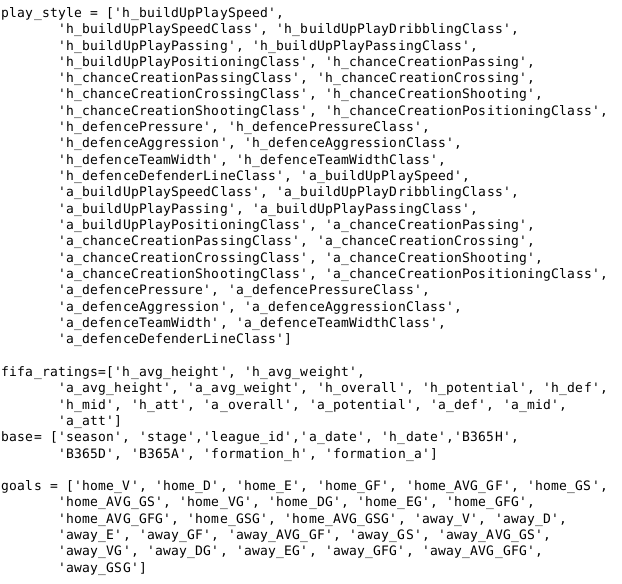
\includegraphics[width=0.45\textwidth]{./04-figuras/features_class.png}
	\caption{Classes com suas respectivas features.}
	\label{fig:class_features}
\end{figure}

Ao todo somam-se 97 features propostas a partir do feature engineering feito com 8791 observações para este conjunto completo. 

Na proxima seção essa features serão avaliadas quando aplicadas a regressão logística, k-neighbors, Random Forest Classifier e Gradient Boosting Classifier.

\section{Experimentos}

 Para a avaliação dos algoritmos será utlizada a métrica multi-class log-loss. Esta métrica é defina pela equação \ref{eq:log_loss}.
 
 \begin{equation}
 \label{eq:log_loss}
 logloss = -\frac{1}{N} \sum_{i}^{N}\sum_{j}^{M}y_{ij}log(p_{ij})
 \end{equation}

onde $N$ é o número de observações, $M$ é o número total de classes alvo no problema, $y_{ij}$ é uma variável binária que é ativa quando sua predição é compatível com a classe $j$ e $p_{ij}$ é a probabilidade dada pelo seu classificador daquela observação $i$ pertencer a classe $j$.

Na figura \ref{fig:logloss} podemos ver o comportamento da multi-class logloss em relação a probabilidade de uma classe.

\begin{figure}[!h]
	\centering
	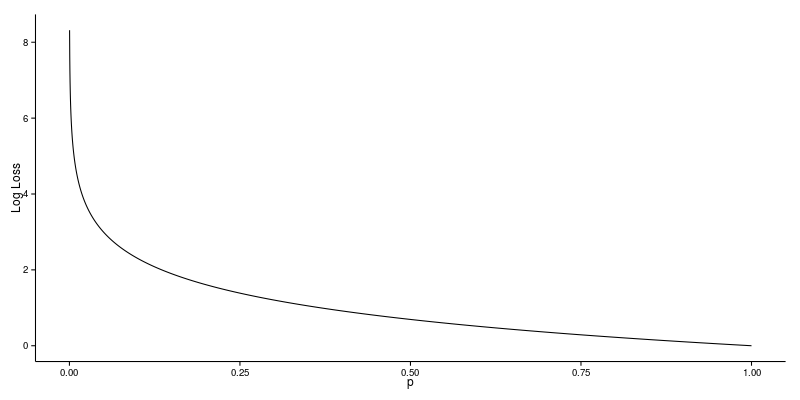
\includegraphics[width=0.45\textwidth]{./04-figuras/log-loss-curve.png}
	\caption{Valor do multiclass logloss vs probabilidade dada a uma classe}
	\label{fig:logloss}
\end{figure}

Acredita-se que essa métrica seja melhor para o problema, visto que ele leva mais em consideração a probabilidade dada para a classe do que o acerto em si. Como futebol é um esporte muito suscetível a aleatóriedades, acredito que essa métrica seja mais adequada do que a acurácia.

Todos os experimentos apresentados nesta seção foram realizados usando kfold cross validation com k=10.

Foram feitas uma normalização min-max, uma gaussiana que proporciona media 0. Foram criadas 3 regressões logisticas, uma para cada grupo de dados para testar se a normalização dos dados afetaria o desempenho. Os dados com normalização min-max apresentaram um logloss de 0.9874, normalização gaussiana 0.9916 e os dados sem normalização 0.9814. Logo descartamos as normalizações no dado.

Agora vamos decidir qual o valor de k, no algoritmo k-neighbors. O gráfico da figura \ref{fig:knn} demonstra que para k=100 atingimos já o valor minimo para o logloss. No gráfico é dado o logloss invertido.

\begin{figure}[!h]
	\centering
	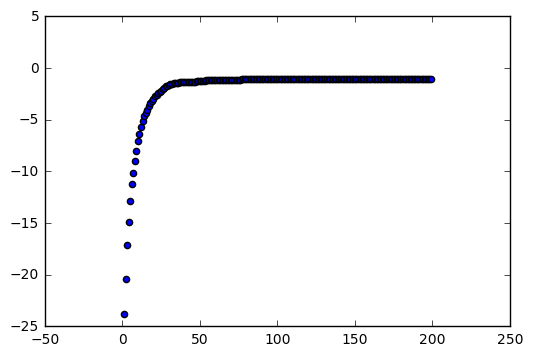
\includegraphics[width=0.45\textwidth]{./04-figuras/knn_k.png}
	\caption{Logloss em função do número de vizinhos}
	\label{fig:knn}
\end{figure}
 Para k = 100, o modelo apresentou um logloss de 1.090.
 
 Para o algoritmo de random forest, aplicamos uma k-fold cross validation para descobrir o melhor valor possível para o número de árvores. O valor de profundidade máximo das árvores foi fixado em 3. O gráfico da figura \ref{fig:rf} demonstra que para k=100 atingimos já o valor minimo para o logloss. No gráfico é dado o logloss invertido.
 
\begin{figure}[!h]
	\centering
	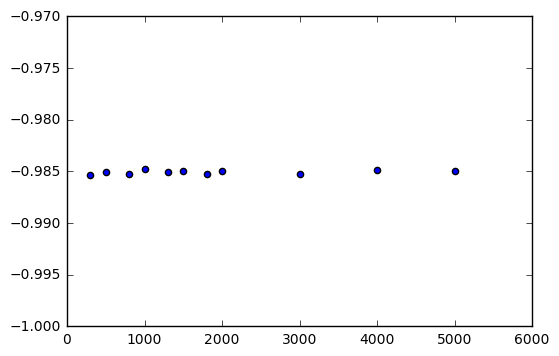
\includegraphics[width=0.45\textwidth]{./04-figuras/random_k.png}
	\caption{Logloss em função do número de árvores}
	\label{fig:knn}
\end{figure}

Podemos observar que temos o menor valor de logloss para k=1000, que foi igual a 0.9850.

O algoritmo Gradient Boosting não teve uma performance satisfatória. Ao fazer o k fold para determinar o melhor valor de estimadores, deu para verificar seu péssimo rendimento. A figura \ref{fig:boosting} demonstra o rendimento. O motivo pelo pouco alcance é que este algoritmo demora muito para ser executado. Como o desempenho foi péssimo comparado aos outros, já terminei a execução.

\begin{figure}[!h]
	\centering
	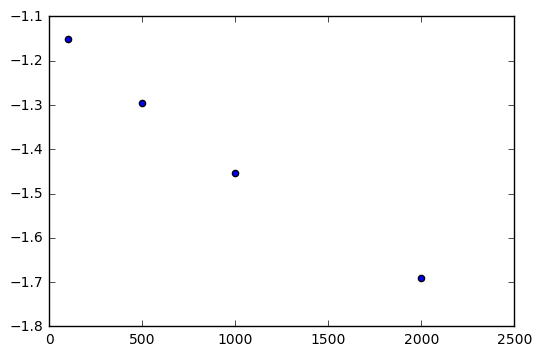
\includegraphics[width=0.45\textwidth]{./04-figuras/gradient_k.png}
	\caption{Logloss em função do número de estimadores para o algoritmo Gradient Boosting.}
	\label{fig:knn}
\end{figure}

Este comportamento é até compreensível, visto que como ele cria uma penalidade pelos erros cometidos pelo último estimador, isso pode atrapalhar muito a predição para o problema do futebol, visto que é um esporte muito suscetível a aleatoriedades.


A tabela \ref{tab:logloss1} apresenta o logloss médio dos modelos apresentado acima.

\begin{table}[!h]
	\centering
	\caption{logloss médio dos algoritmos usando os dados com feature engineering}
	\label{tab:logloss1}
	\begin{tabular}{c|c}
		& logloss médio \\ \hline
		Regressão Logística & 0.9814        \\ \hline
		K-Neighbors         & 1.090         \\ \hline
		Random Forest       & 0.9850        \\ \hline
		Gradient Boosting   & 1.170        
	\end{tabular}
\end{table}


Vamos agora testar os 3 modelos com melhores médias com as diferentes combinações de classes de features. A tabela \ref{tab:comb} apresenta o logloss médio dos algoritmos com as combinação das classes de features.

Como podemos observar na tabela \ref{tab:comb} a classe Play\_Style aumenta o logloss médio dos algoritmos. Podemos observar também que o algoritmo Regressão Logística apresentou um melhor desempenho médio.
\begin{table}[!h]
	\centering
	\caption{logloss médio de cada algoritmo para cada classe de entrada;}
	\label{tab:comb}
	\begin{tabular}{c|c|c|c}
		& Reg. Log. & K-NN   & R. Forest \\ \hline
		Base                   & 0.9735    & 1.0364 & 1.0278    \\ \hline
		Goals                  & 1.0331    & 1.0378 & 1.063     \\ \hline
		Ratings                & 0.9849    & 0.9940 & 1.0097    \\ \hline
		Style                  & 1.0061     & 1.0644 & 1.0883    \\ \hline
		Base + Goals           & 0.9741    & 1.0494 & 0.9939    \\ \hline
		Base + Ratings         & 0.9733    & 1.0090 & 0.9931    \\ \hline
		Base + Style           & 0.9793    & 1.0700  & 1.0034    \\ \hline
		Goals + Ratings        & 0.9868    & 0.9926 & 0.9974    \\ \hline
		Goals + Style          & 1.0390    & 1.0400 & 1.0446    \\ \hline
		Ratings + Style        & 0.9981    & 1.0239 & 1.0036    \\ \hline
		Base+Goals+Rating      & 0.9747    & 1.0263 & 0.9902    \\ \hline
		Base+Goals+Style       & 0.9816    & 1.0604 & 0.9930    \\ \hline
		Base +Rating + Style   & 0.9802    & 1.0478 & 0.9921    \\ \hline
		Goals + Rating + Style & 1.0007    & 1.0186 & 1.0006   
	\end{tabular}
\end{table}

Partindo para o conceito da filtragem dos dados apresentado por Cheng et al. \cite{cheng2003new}, separei os dados em mandante forte quando a diferença de overall médio do mandante é superior ou igual a 3 unidades em relação ao visitante. Caso o overall do visitante seja maior ou igual ao mandante em 3 unidades esses jogos são filtrados como visitante forte. Se não entrar em nenhum desses filtros, entra para o filtro de jogos com equipes em niveis iguais.

O algoritmo que apresentou melhor desempenho para o mandante forte foi Regressão Logistica com as features da classe Base. O logloss médio foi de 0.8150.

Para os visitantes fortes o modelo que apresentou melhor desempenho foi  Regressão Logistica com as features da classe Base. O logloss médio foi de 1.0036.

Para os jogos em níveis iguais o algoritmo que apresentou melhor desempenho médio foi Regressão Logistica com as features da classe Base. O logloss médio foi de 1.0550.

Separando 33\% das observações para o teste e criando o modelo híbrido proposto por Cheng et al. \cite{cheng2003new}, obtemos o 1.2853 como logloss médio.

\section{Conclusão}

Para predição de jogos de futebol, o algoritmo de regressão linear apresentou melhor desempenho médio. 

Como predição de jogos de futebol é uma tarefa muito complexa, consegui consolidar conceitos complexos apresentados em sala de aula.

Como trabalhos futuros, criar sistemas mais simples envolvendo futebol que possam sirvir como features para a predição de futebol é o próximo passo que irei seguir.
% In the unusual situation where you want a paper to appear in the
% references without citing it in the main text, use \nocite

\bibliography{example_paper}
\bibliographystyle{icml2015}

\end{document} 


